\documentclass[article]{article}

% Packages
\usepackage[utf8]{inputenc}
\usepackage[T1]{fontenc}
\usepackage{geometry}
\usepackage{graphicx}
\usepackage{booktabs}
\usepackage{array}
\usepackage{longtable}
\usepackage{float}
\usepackage{hyperref}
\usepackage{caption}
\usepackage{subcaption}
\usepackage{amsmath}
\usepackage{amssymb}
\usepackage{xcolor}
\usepackage{tabularx}

% Page setup
\geometry{a4paper, margin=2.5cm}
\setlength{\parindent}{0pt}
\setlength{\parskip}{6pt}

% Hyperref setup
\hypersetup{
    colorlinks=true,
    linkcolor=blue,
    filecolor=magenta,      
    urlcolor=cyan,
    citecolor=red
}

% Title
\title{EVM Semantics Evaluation Results}
\author{perfx}
\date{\today}

\begin{document}

\maketitle

\tableofcontents
\newpage

\section{Tables}

\subsection{Opcode Summarization Results}\label{tab:step3_opcode_list}

\begin{table}[htbp]
\centering
\caption{Opcode Summarization Results}
\label{tab:step3_opcode_list}
\begin{tabularx}{\textwidth}{XXX}
\toprule
Category & Successful Opcodes & Failed Opcodes \\
\midrule
Arith. \& Bit. & SUB, DIV, ADD, MOD, SMOD, SDIV, ADDMOD, MULMOD, SIGNEXTEND, AND, EVMOR, XOR, NOT, SHL, BYTE, SHR & MUL, EXP, SAR \\
Comparison & LT, GT, SLT, EQ, SGT, ISZERO &  \\
Flow Control & STOP, PC, JUMPDEST, INVALID, RETURN, REVERT, UNDEFINED & JUMP, JUMPI \\
Stack & POP, PUSHZERO, PUSH1-32, DUP1-16, SWAP1-16 &  \\
Memory & MLOAD, MSTORE, MSTORE8, MSIZE, MCOPY &  \\
Storage & SLOAD, SSTORE &  \\
Trans. Storage & TLOAD, TSTORE &  \\
Environment & COINBASE, BLOCKHASH, TIMESTAMP, NUMBER, PREVRANDAO, DIFFICULTY, GASLIMIT, CHAINID & BASEFEE \\
Context & ADDRESS, ORIGIN, CALLER, CALLDATALOAD, CALLDATASIZE, CALLDATACOPY, CODESIZE, CODECOPY, GASPRICE, BALANCE, RETURNDATASIZE, RETURNDATACOPY, SELFBALANCE, GAS & CALLVALUE, EXTCODECOPY, EXTCODEHASH, EXTCODESIZE \\
System & LOG0-4 & SHA3 \\
Contract &  & CALL, CALLCODE, CREATE, CREATE2, DELEGATECALL, SELFDESTRUCT, STATICCALL \\
\bottomrule
\end{tabularx}
\end{table}

\newpage

\subsection{Statistics of Opcode Summarization}\label{tab:step3_category_statistics}

\begin{table}[htbp]
\centering
\caption{Statistics of Opcode Summarization}
\label{tab:step3_category_statistics}
\begin{tabular}{lrrrlllr}
\toprule
Category & \# & G. Succ. & V. Succ. & G. Time (s) & V. Time (s) & Steps & \$\textbackslash\{\}Delta\$ Steps \\
\midrule
Arith. \& Bit. & 19 & 84.2\% & 100.0\% & 52.0 & 161.9 & 8.0 & 87.5\% \\
Comparison & 6 & 100.0\% & 100.0\% & 64.4 & 94.8 & 9.5 & 89.5\% \\
Flow Control & 9 & 77.8\% & 100.0\% & 52.1 & 106.7 & 6.8 & 85.4\% \\
Stack & 5 & 100.0\% & 100.0\% & 77.4 & 110.6 & 9.3 & 89.2\% \\
Memory & 5 & 100.0\% & 100.0\% & 78.3 & 106.7 & 10.1 & 90.1\% \\
Storage & 2 & 100.0\% & 100.0\% & 97.9 & 693.5 & 10.5 & 90.5\% \\
Trans. Storage & 2 & 100.0\% & 100.0\% & 72.9 & 107.2 & 9.0 & 88.9\% \\
Environment & 9 & 88.9\% & 100.0\% & 65.3 & 374.5 & 8.4 & 88.2\% \\
Context & 18 & 77.8\% & 100.0\% & 66.6 & 428.6 & 7.8 & 87.2\% \\
System & 2 & 50.0\% & 100.0\% & 41.8 & 103.3 & 5.0 & 80.0\% \\
Contract & 7 & 0.0\% & 0.0\% & 0.0 & 0.0 & 0.0 & 0.0\% \\
Total & 84 & 78.6\% & 100.0\% & 73.3 & 233.6 & 9.6 & 89.6\% \\
\bottomrule
\end{tabular}
\end{table}

\newpage

\section{Charts}

\subsection{Concrete Execution Performance Comparison}\label{fig:concrete_performance_comparison}

\begin{figure}[H]
\centering
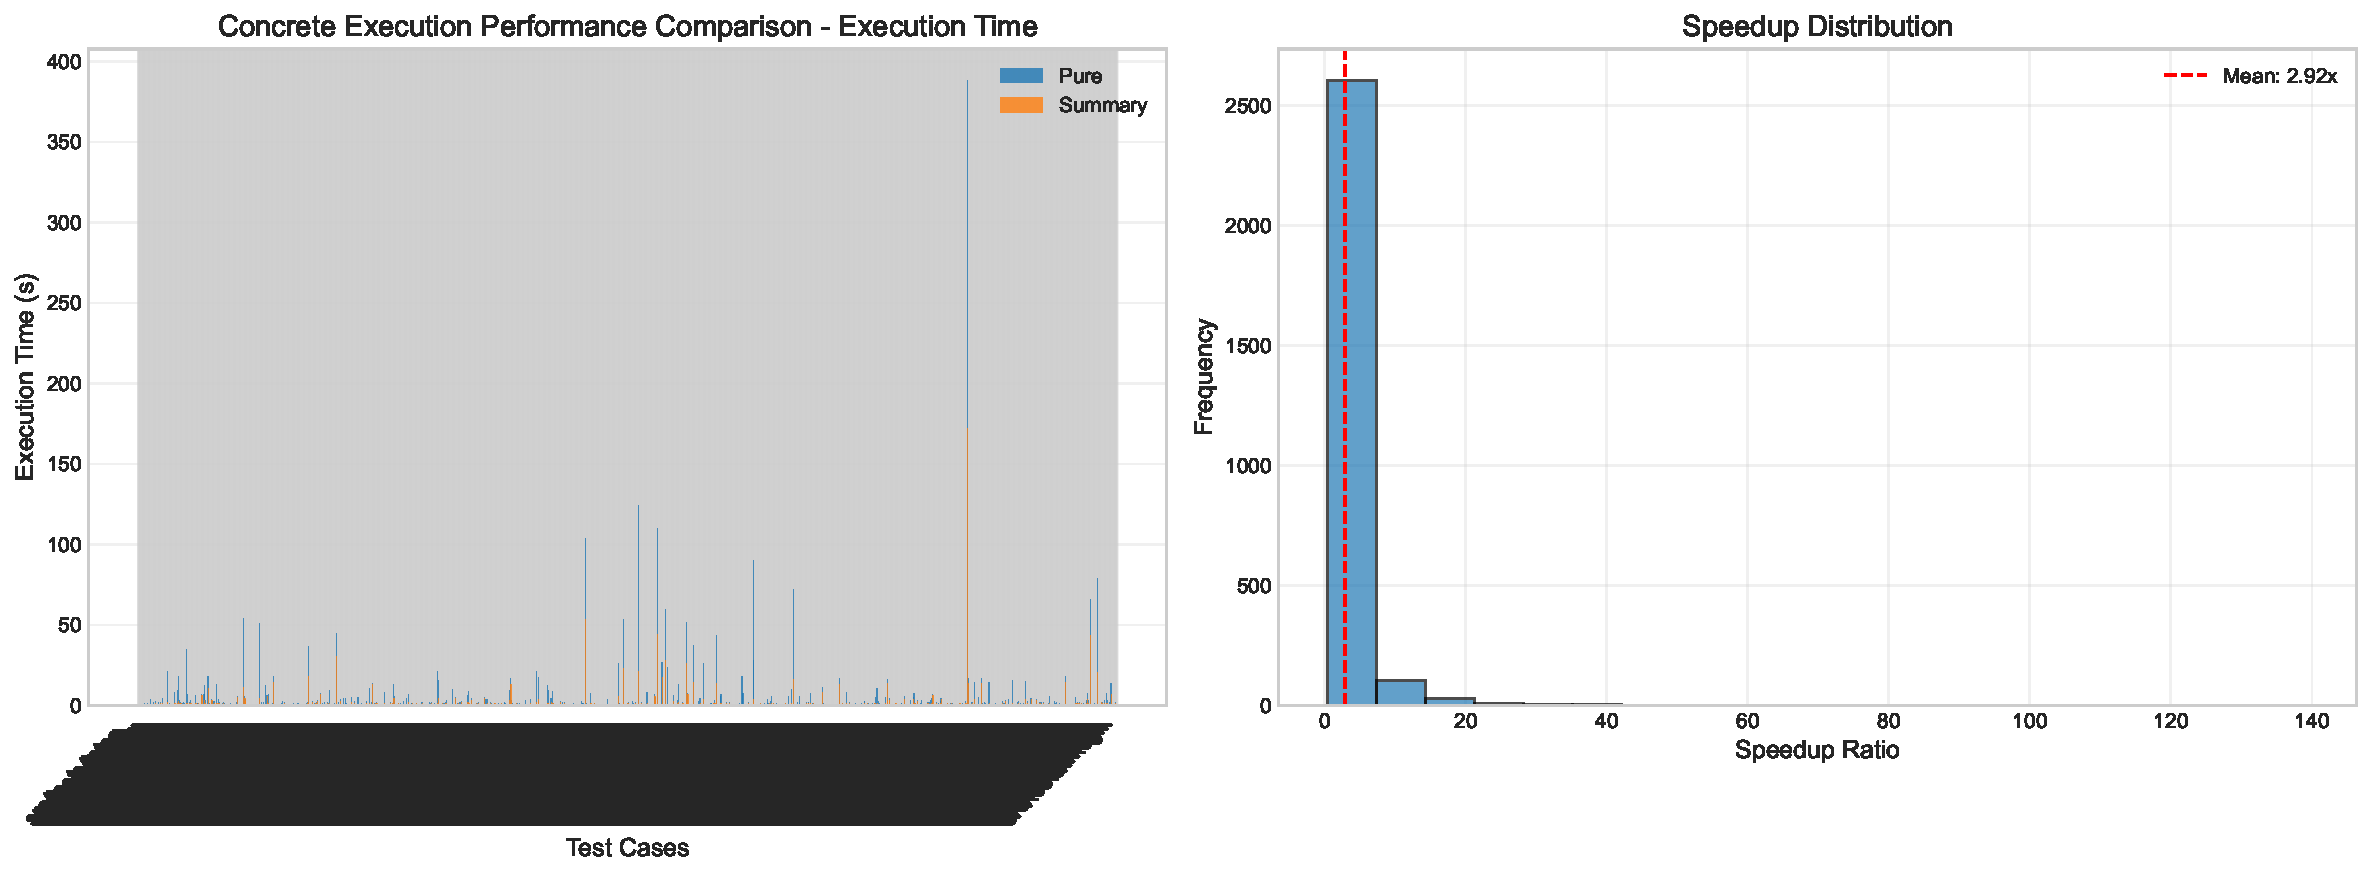
\includegraphics[width=0.8\textwidth]{charts/concrete_performance_comparison.pdf}
\caption{Concrete Execution Performance Comparison}
\label{fig:concrete_performance_comparison}
\end{figure}

\newpage

\subsection{Concrete Execution Performance Distribution}\label{fig:concrete_performance_distribution}

\begin{figure}[H]
\centering
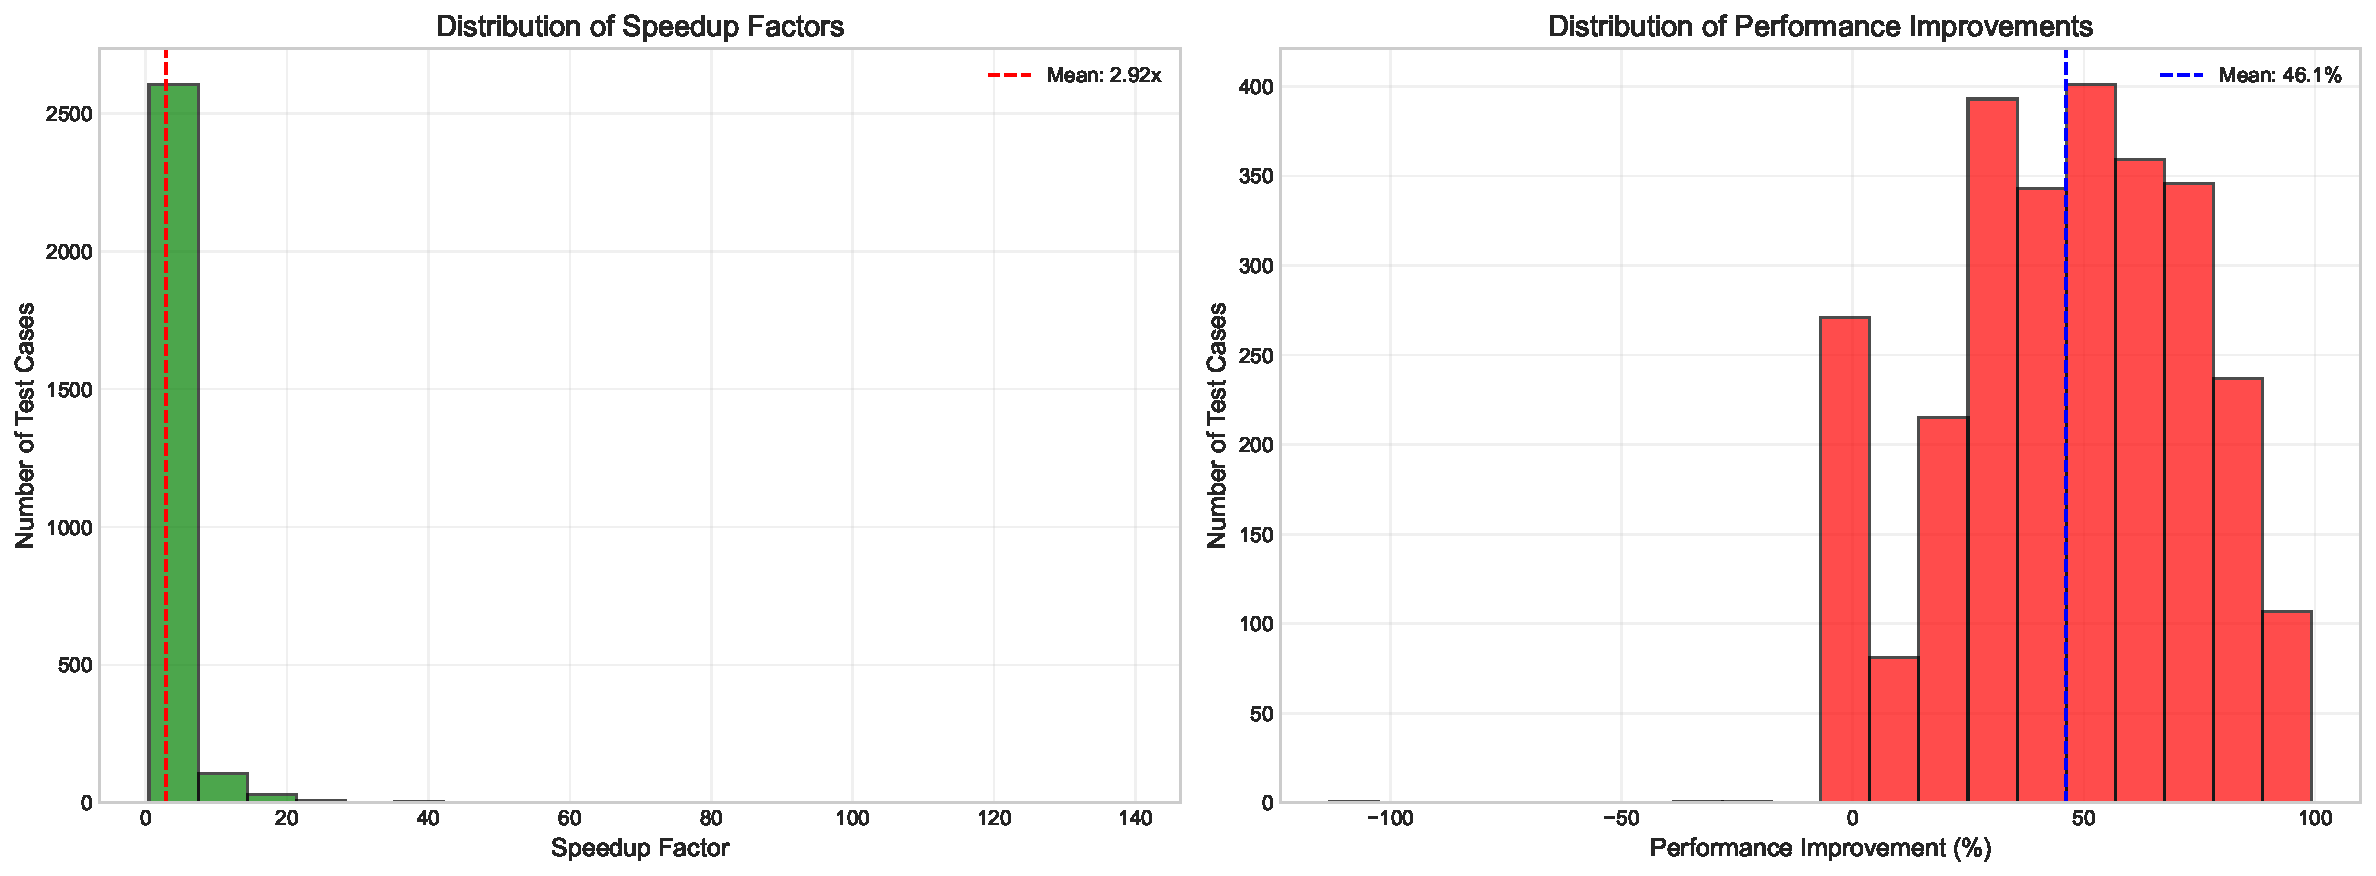
\includegraphics[width=0.8\textwidth]{charts/concrete_performance_distribution.pdf}
\caption{Concrete Execution Performance Distribution}
\label{fig:concrete_performance_distribution}
\end{figure}

\newpage

\subsection{Performance Comparison: Original vs Summarized Semantics}\label{fig:concrete_performance_scatter}

\begin{figure}[H]
\centering
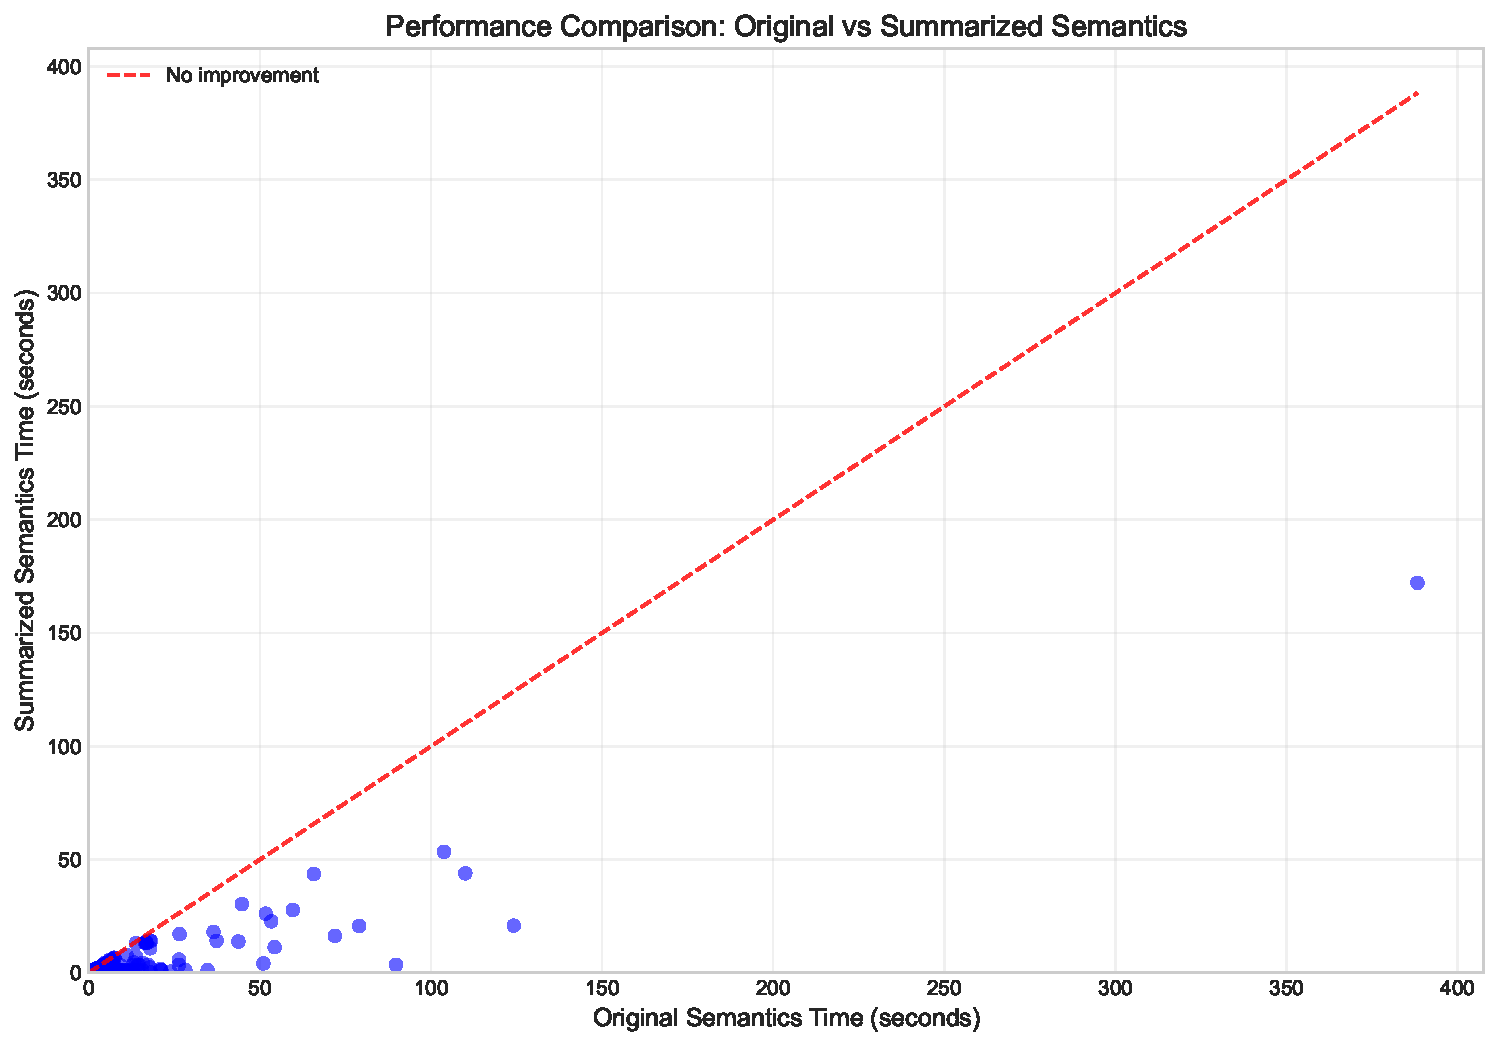
\includegraphics[width=0.8\textwidth]{charts/concrete_performance_scatter.pdf}
\caption{Performance Comparison: Original vs Summarized Semantics}
\label{fig:concrete_performance_scatter}
\end{figure}

\newpage

\subsection{Top 20 Test Cases by Performance Improvement}\label{fig:concrete_test_case_improvement}

\begin{figure}[H]
\centering
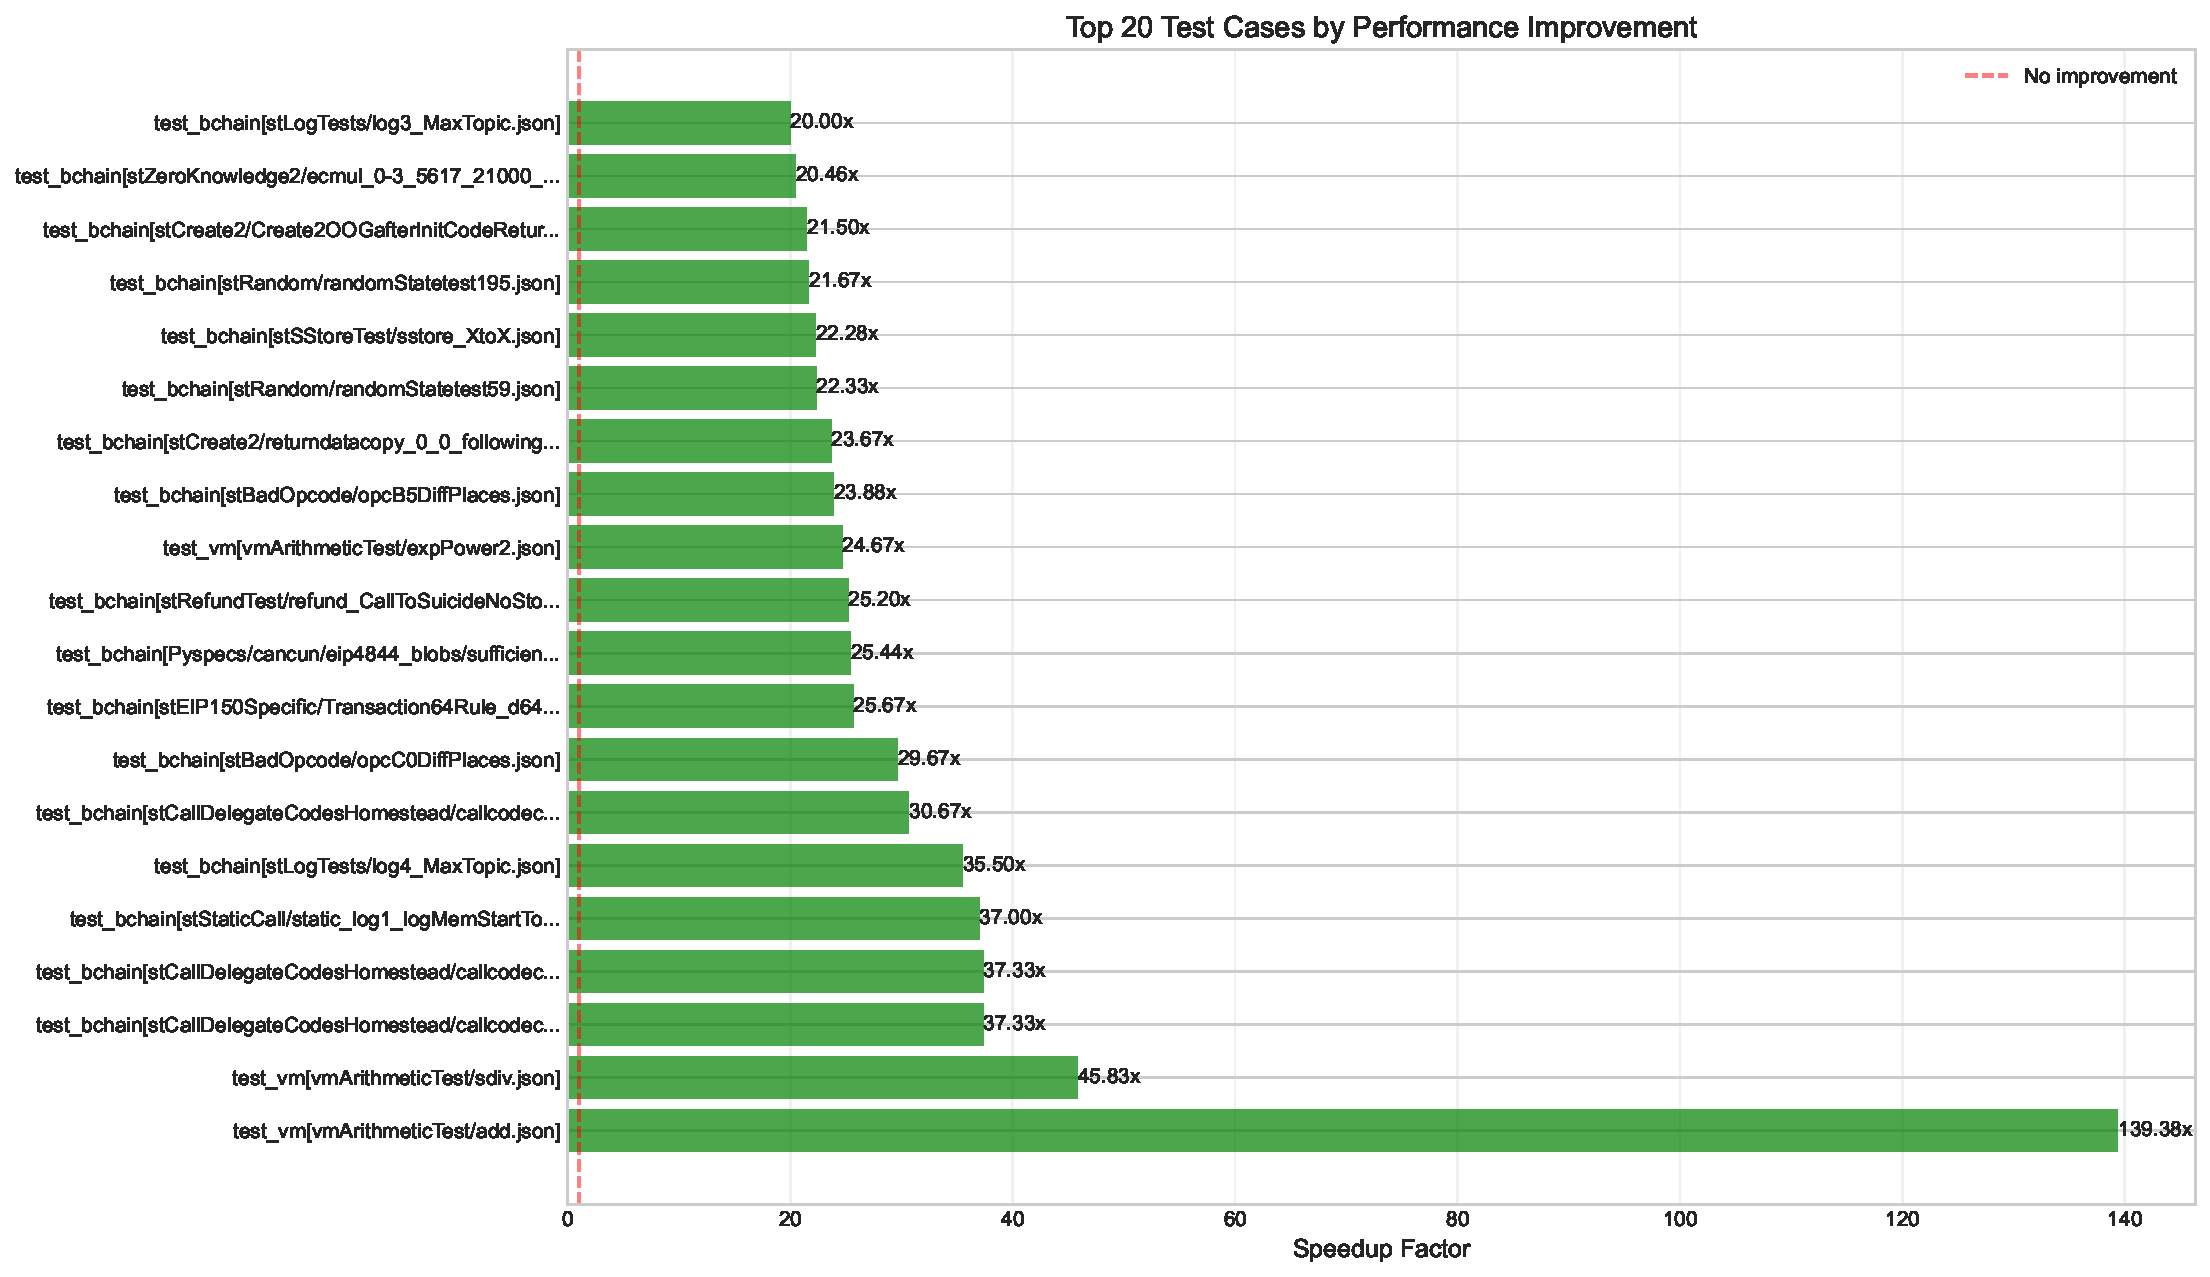
\includegraphics[width=0.8\textwidth]{charts/concrete_test_case_improvement.pdf}
\caption{Top 20 Test Cases by Performance Improvement}
\label{fig:concrete_test_case_improvement}
\end{figure}

\newpage

\subsection{Symbolic Execution Performance Comparison: Original vs Summarized Semantics}\label{fig:symbolic_performance_scatter}

\begin{figure}[H]
\centering
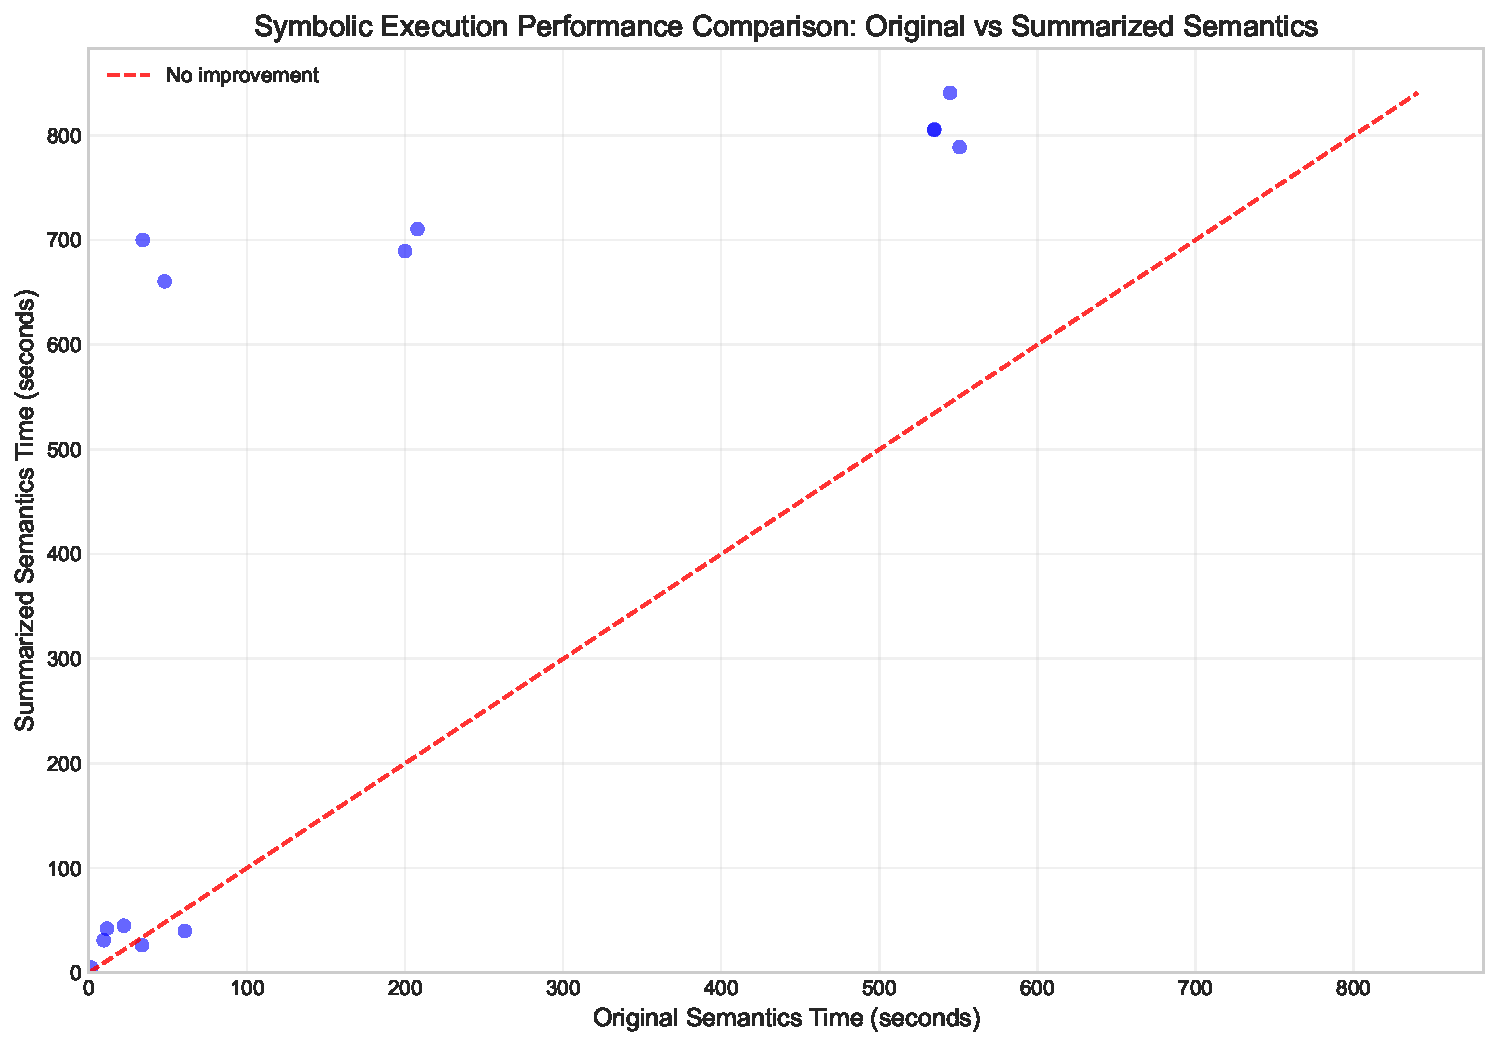
\includegraphics[width=0.8\textwidth]{charts/symbolic_performance_scatter.pdf}
\caption{Symbolic Execution Performance Comparison: Original vs Summarized Semantics}
\label{fig:symbolic_performance_scatter}
\end{figure}

\newpage

\subsection{Top Symbolic Test Cases by Performance Improvement}\label{fig:symbolic_test_case_improvement}

\begin{figure}[H]
\centering
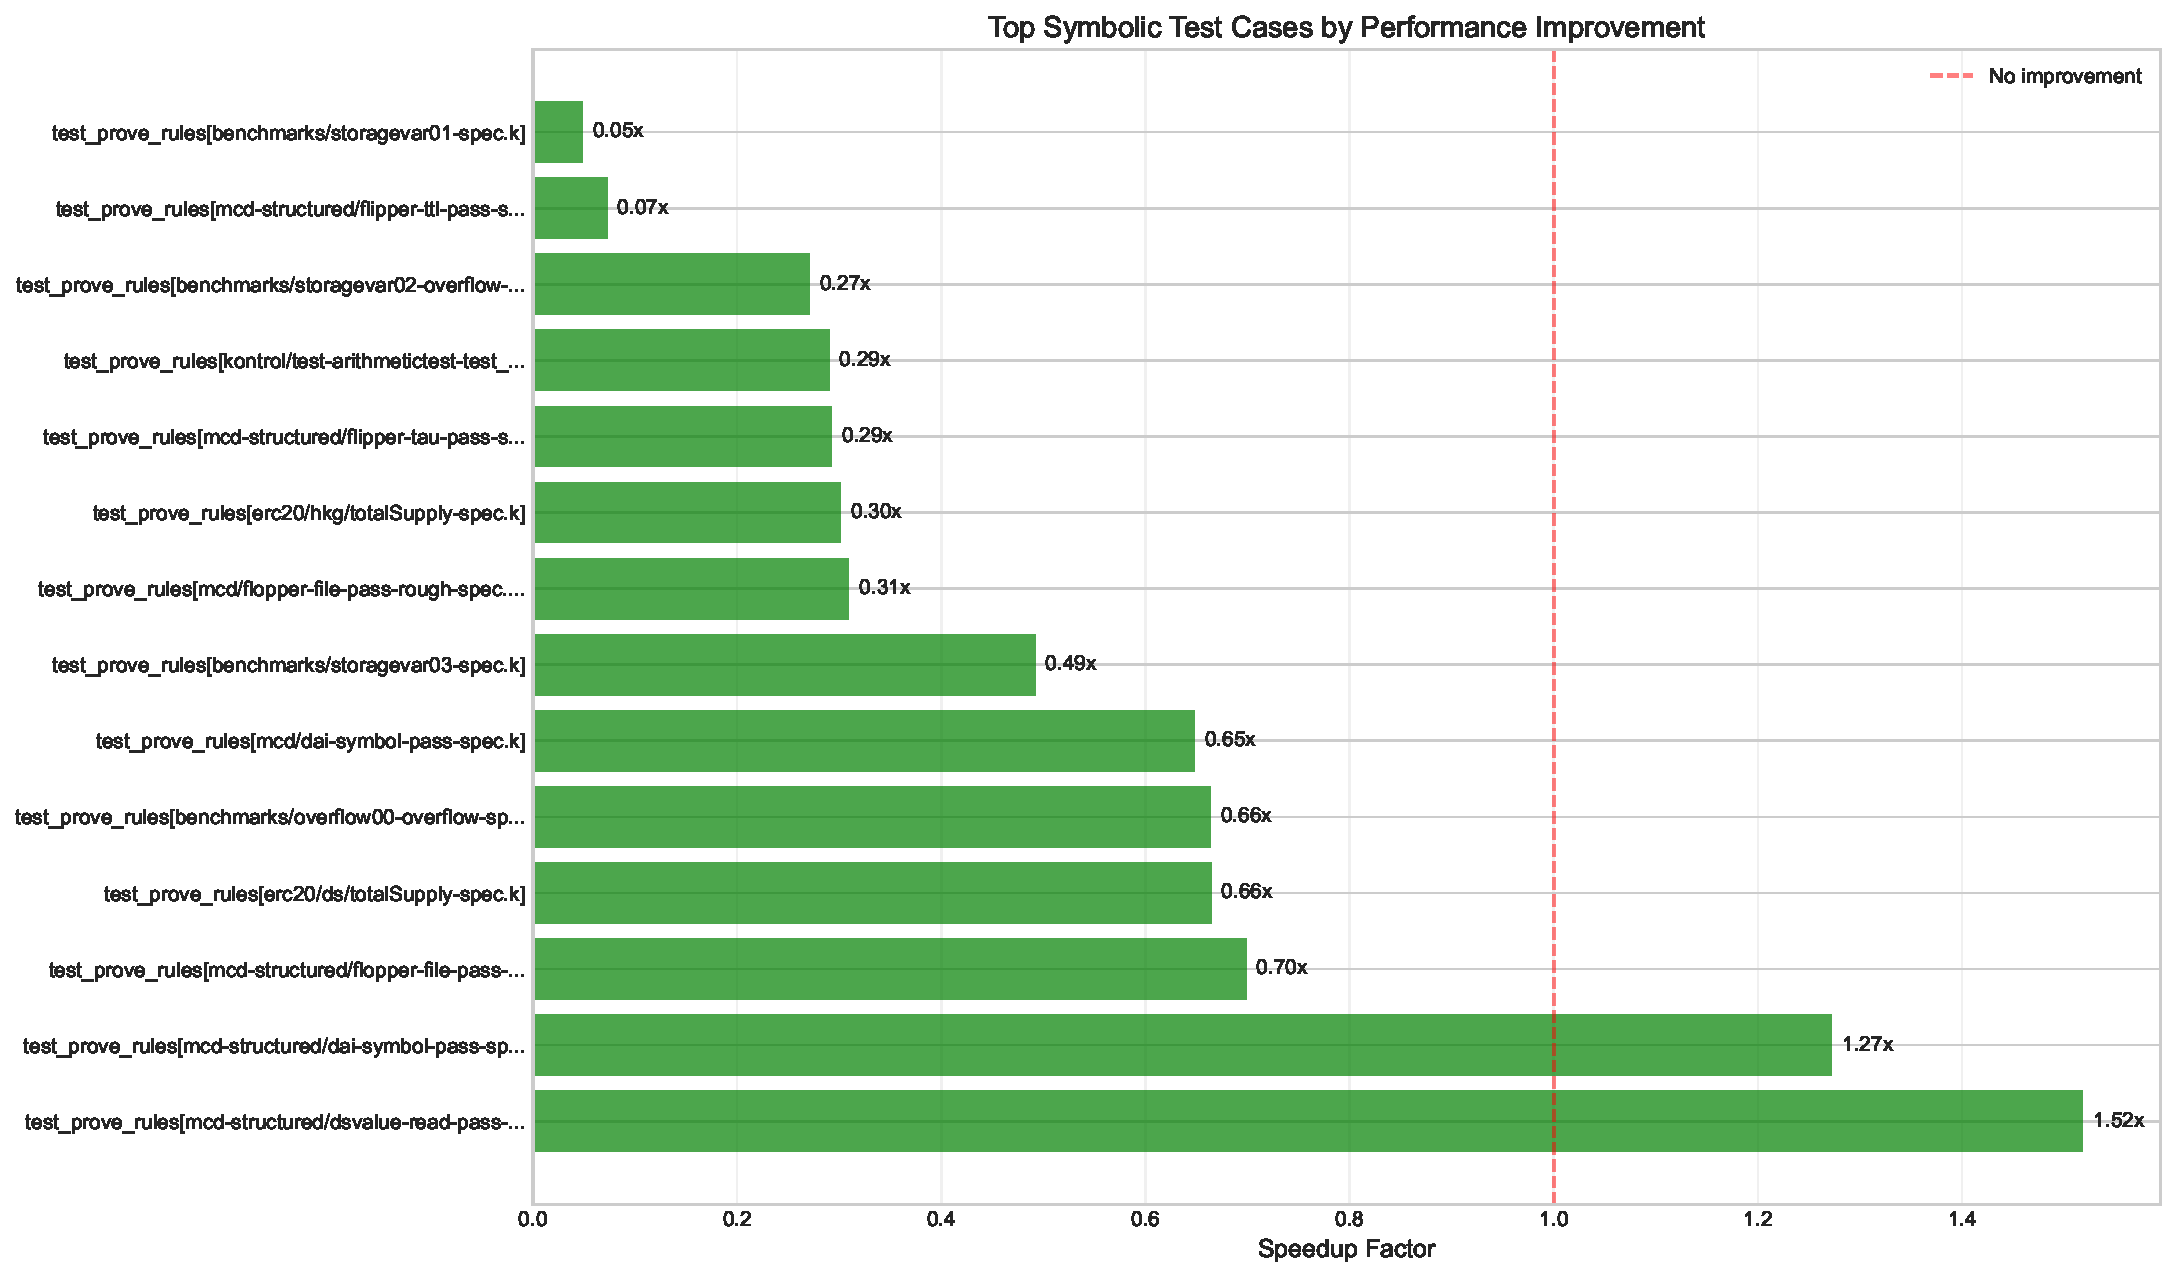
\includegraphics[width=0.8\textwidth]{charts/symbolic_test_case_improvement.pdf}
\caption{Top Symbolic Test Cases by Performance Improvement}
\label{fig:symbolic_test_case_improvement}
\end{figure}

\newpage

\subsection{Symbolic Execution Performance Comparison (Booster): Original vs Summarized Semantics}\label{fig:symbolic_booster_performance_scatter}

\begin{figure}[H]
\centering
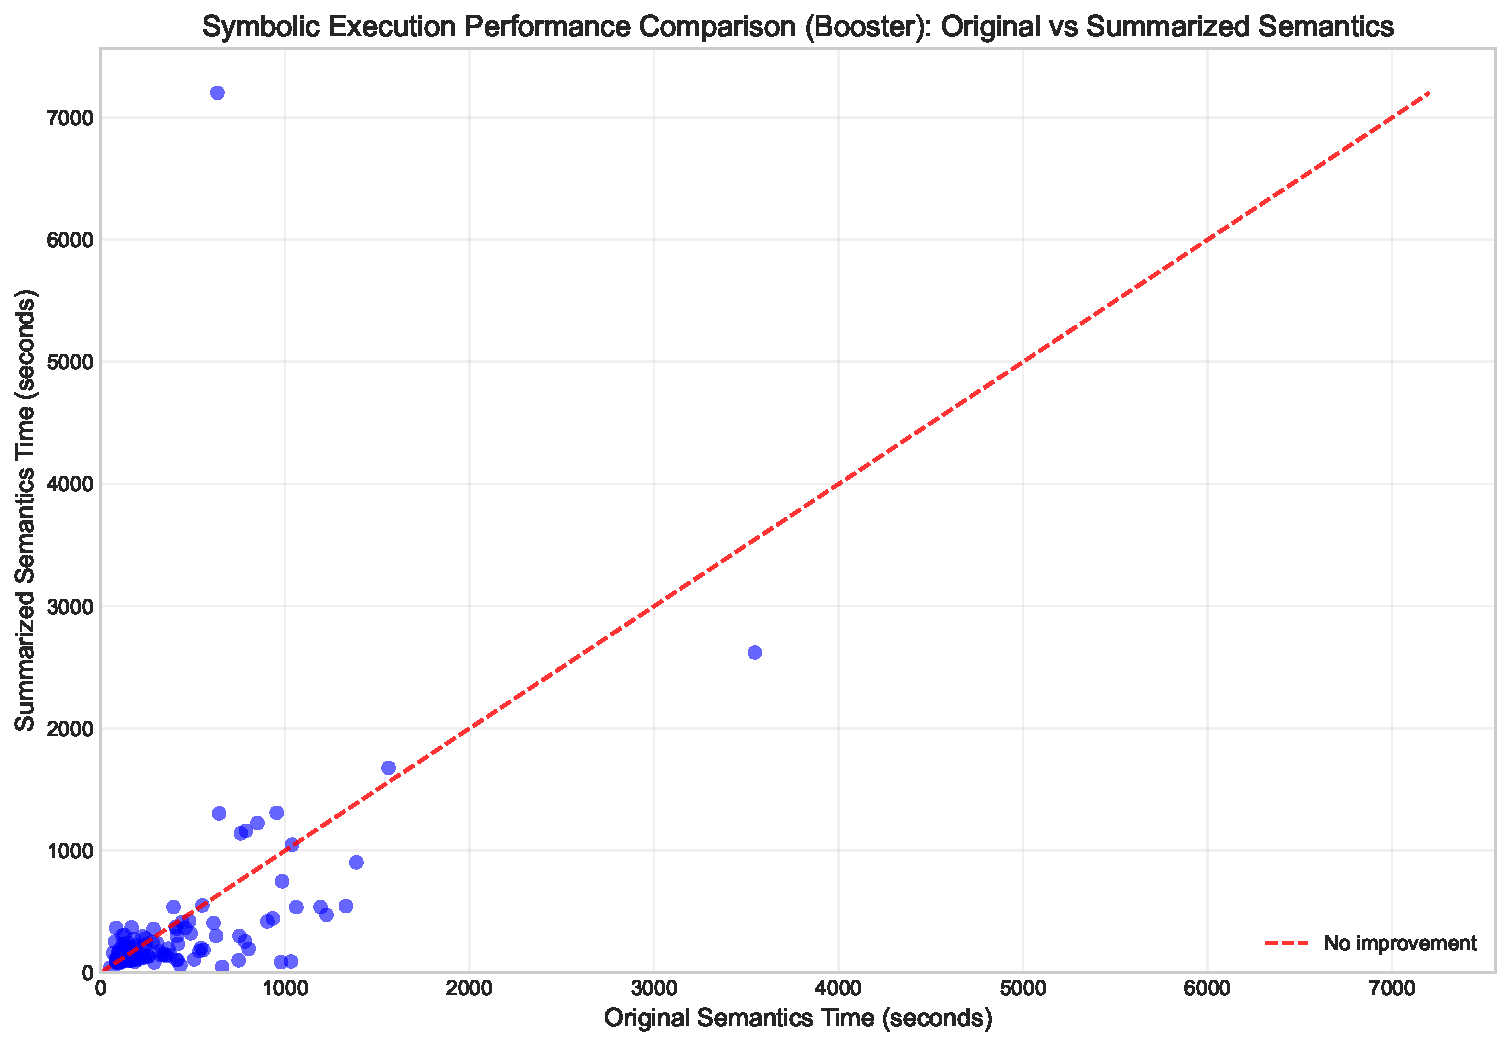
\includegraphics[width=0.8\textwidth]{charts/symbolic_booster_performance_scatter.pdf}
\caption{Symbolic Execution Performance Comparison (Booster): Original vs Summarized Semantics}
\label{fig:symbolic_booster_performance_scatter}
\end{figure}

\newpage

\subsection{Top Symbolic Test Cases by Performance Improvement (Booster)}\label{fig:symbolic_booster_test_case_improvement}

\begin{figure}[H]
\centering
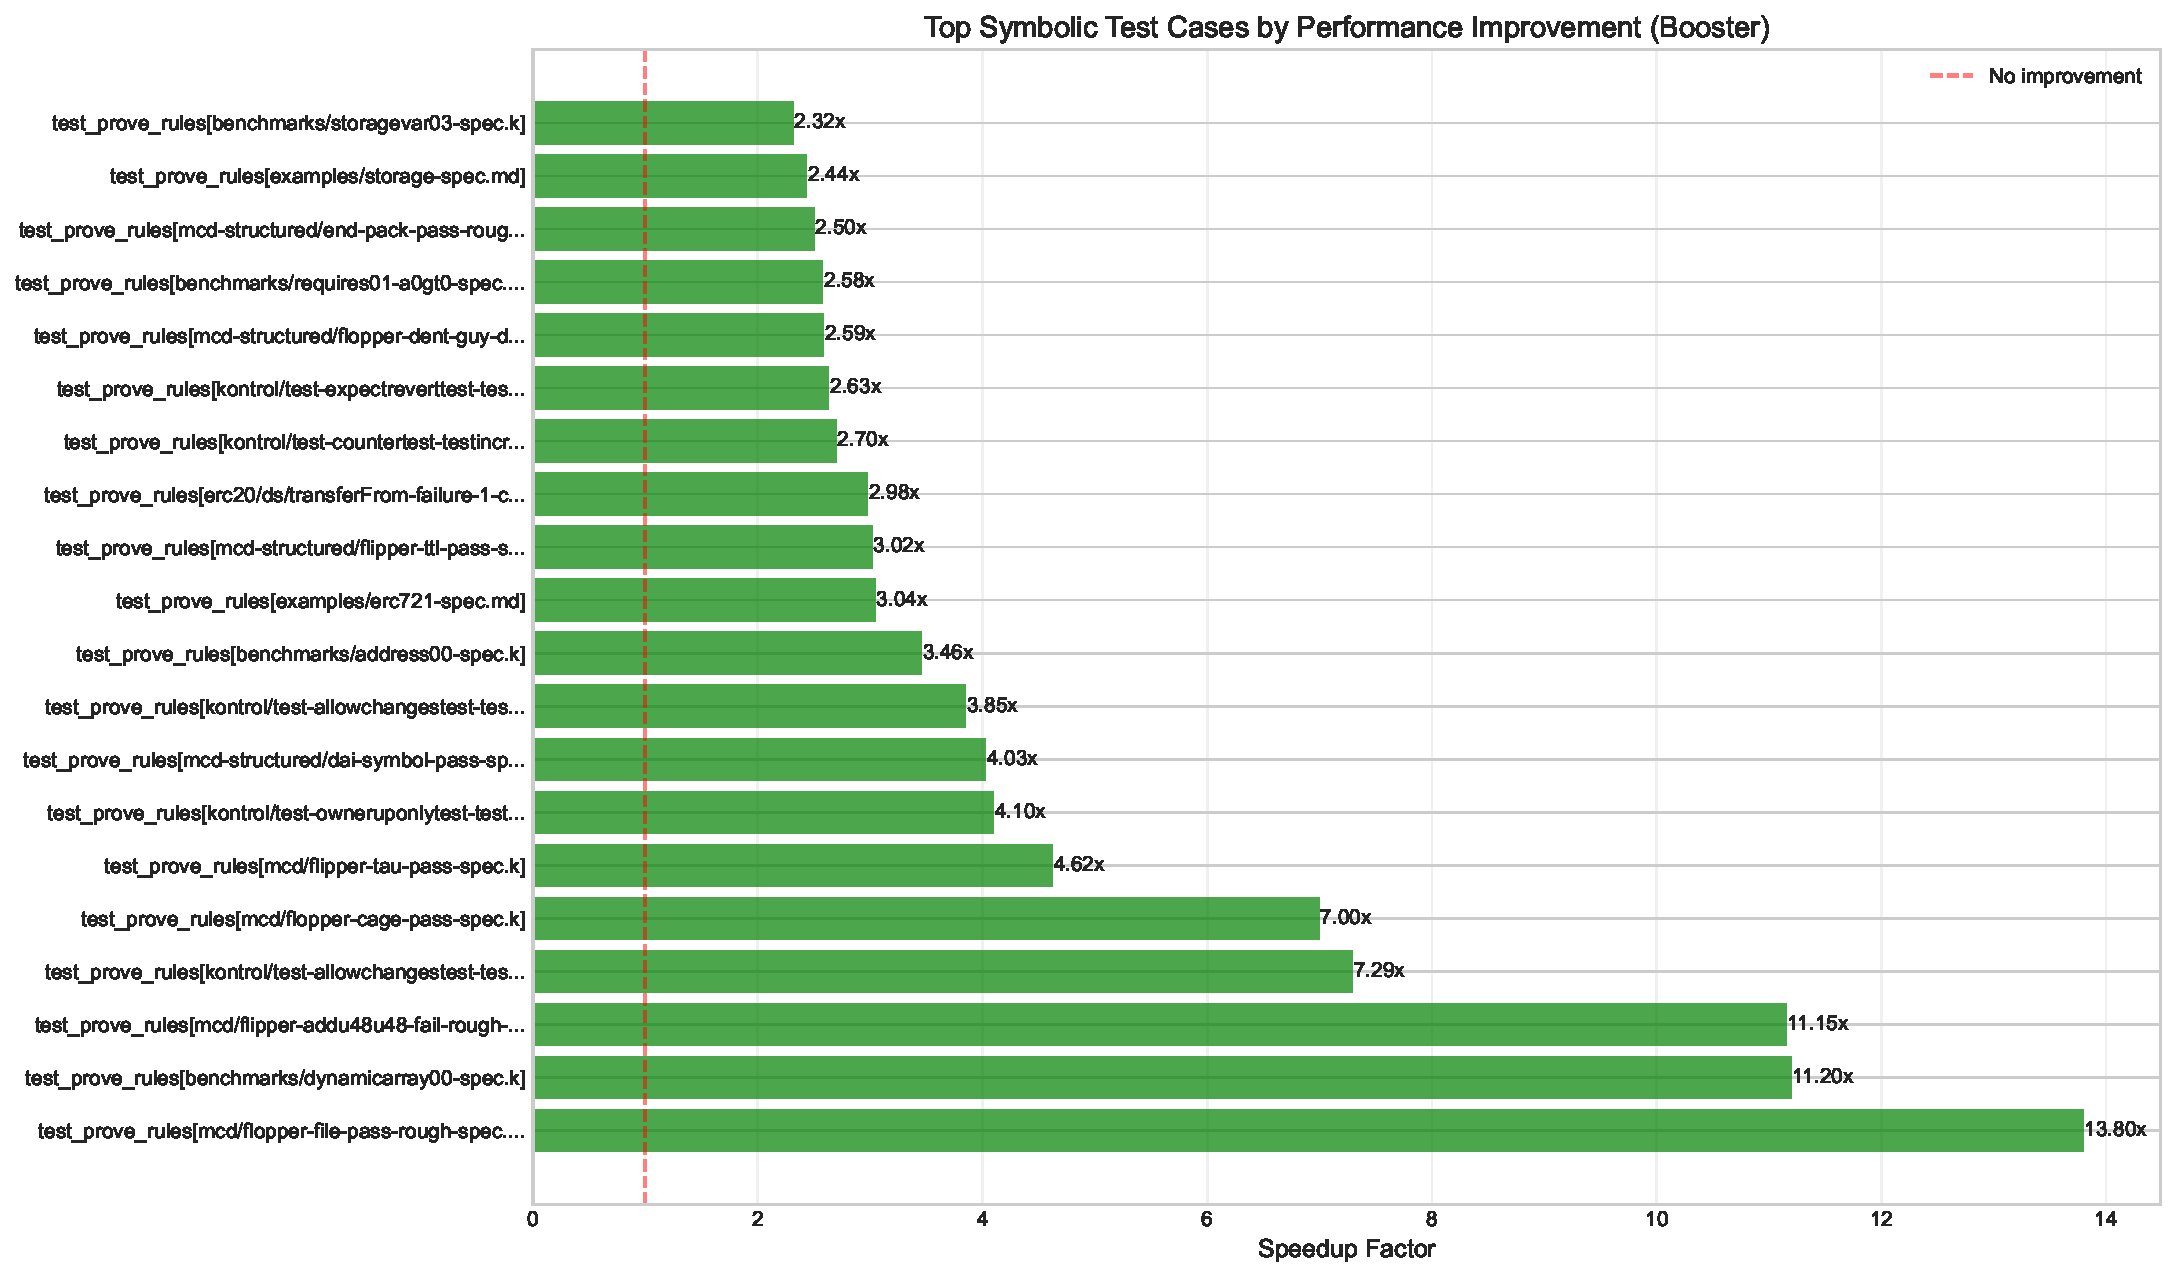
\includegraphics[width=0.8\textwidth]{charts/symbolic_booster_test_case_improvement.pdf}
\caption{Top Symbolic Test Cases by Performance Improvement (Booster)}
\label{fig:symbolic_booster_test_case_improvement}
\end{figure}

\newpage

\subsection{Symbolic Execution Performance Comparison (Summaries): Original vs Summarized Semantics}\label{fig:symbolic_summaries_performance_scatter}

\begin{figure}[H]
\centering
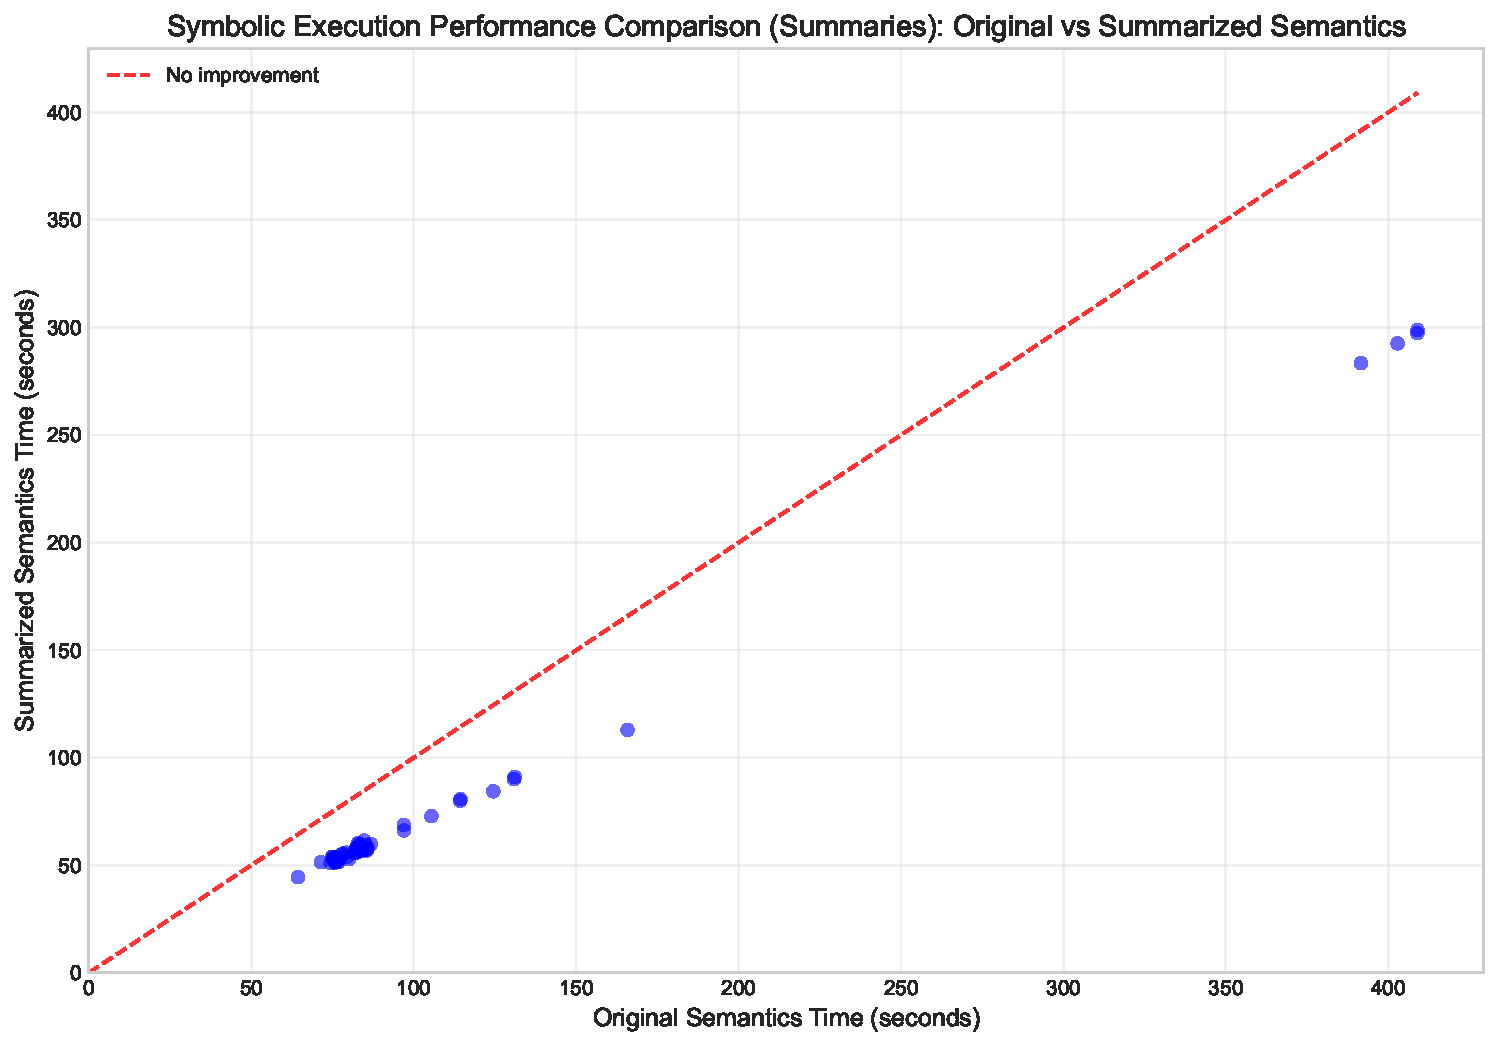
\includegraphics[width=0.8\textwidth]{charts/symbolic_summaries_performance_scatter.pdf}
\caption{Symbolic Execution Performance Comparison (Summaries): Original vs Summarized Semantics}
\label{fig:symbolic_summaries_performance_scatter}
\end{figure}

\newpage

\subsection{Top Symbolic Test Cases by Performance Improvement (Summaries)}\label{fig:symbolic_summaries_test_case_improvement}

\begin{figure}[H]
\centering
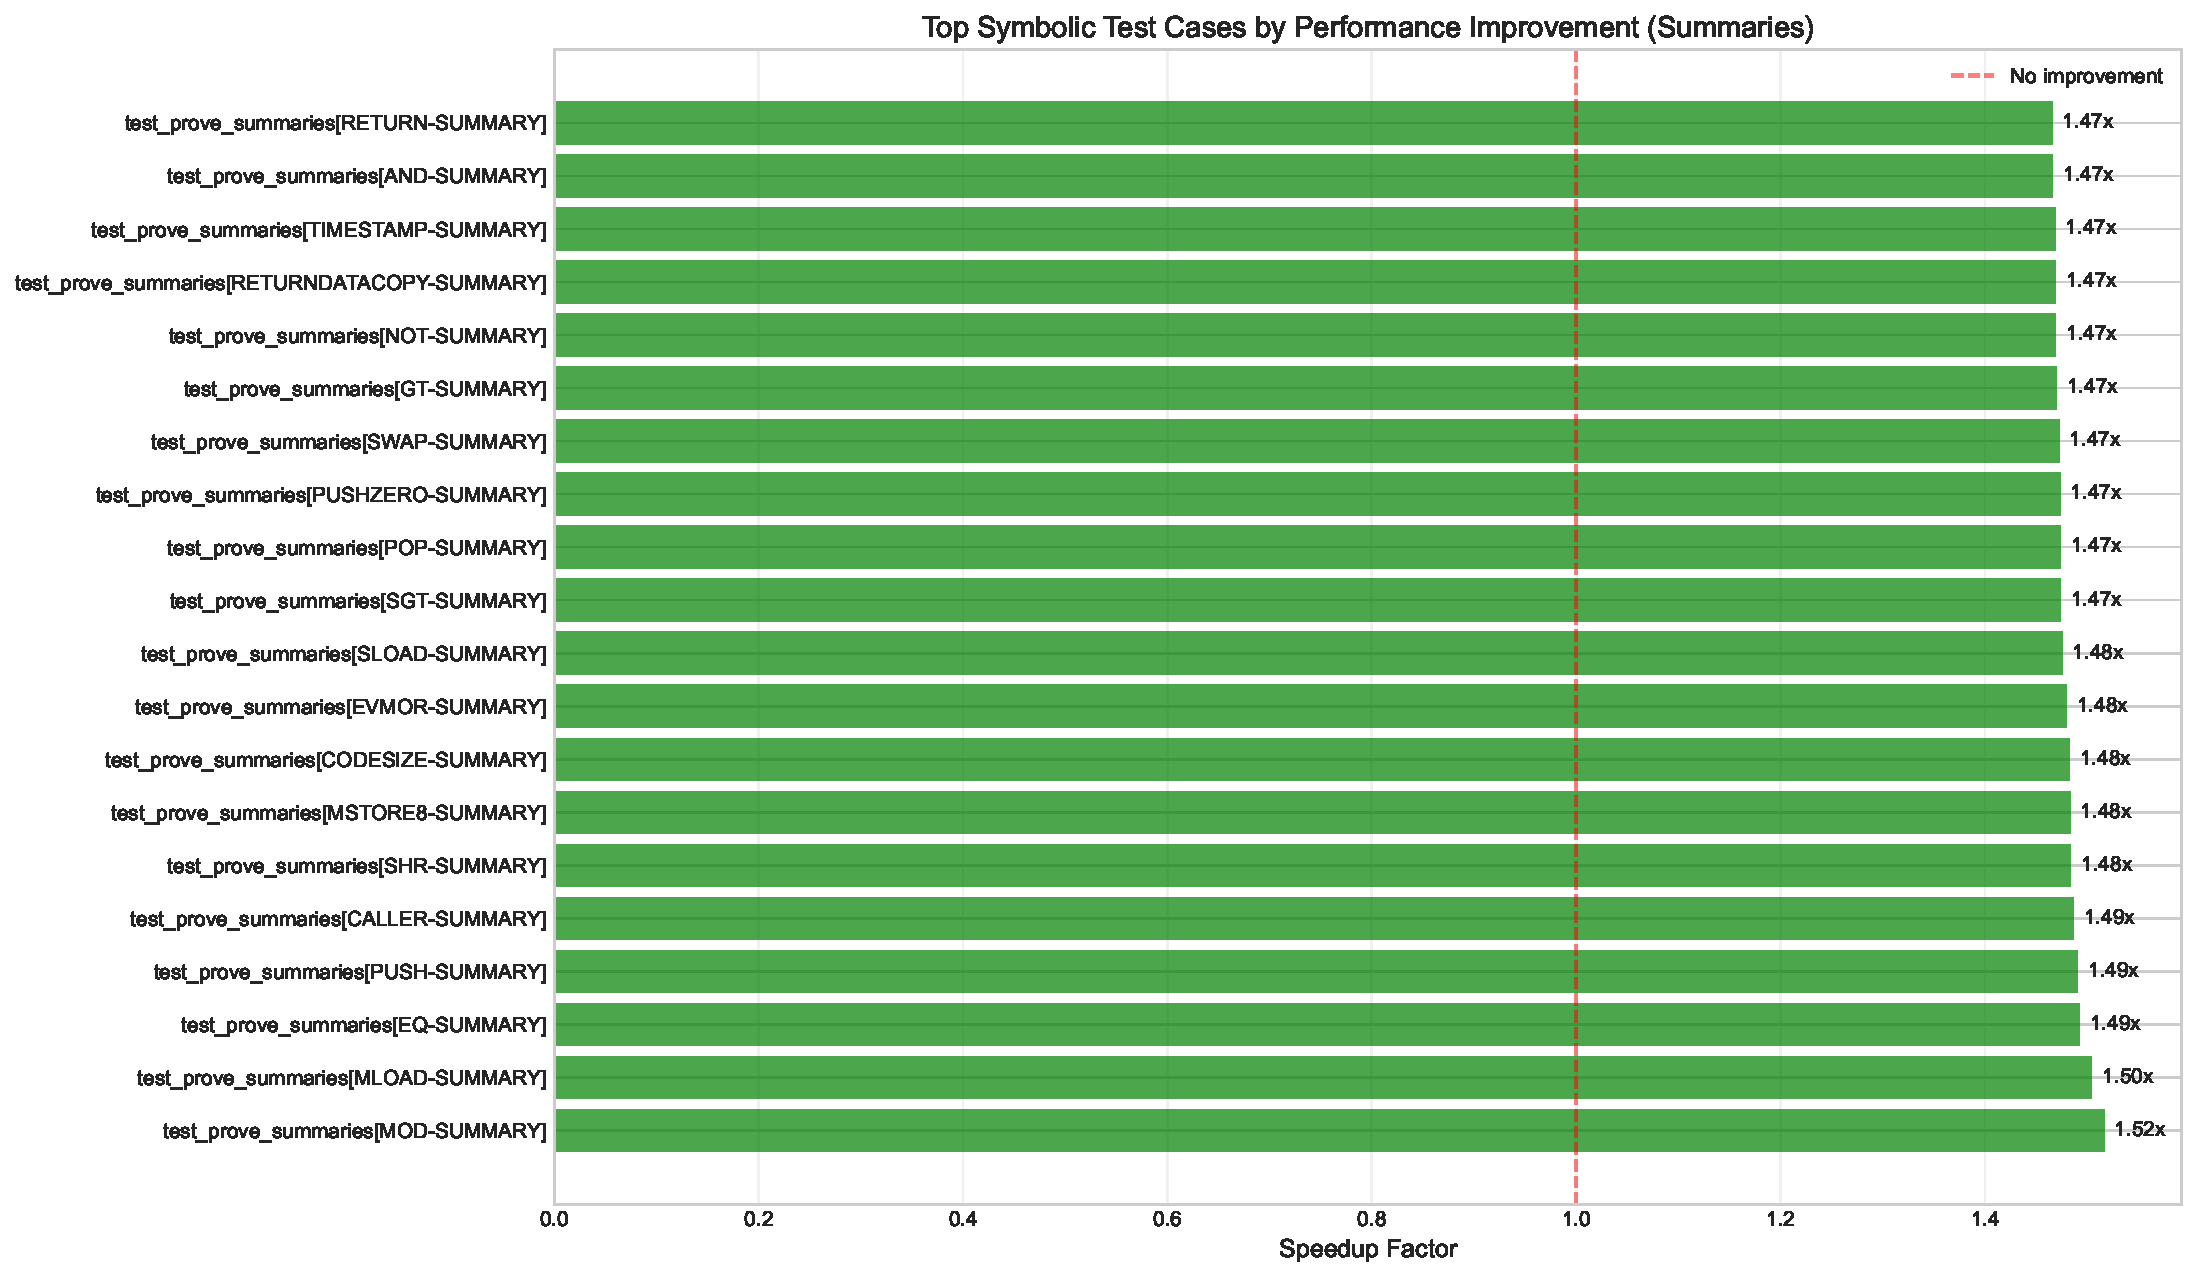
\includegraphics[width=0.8\textwidth]{charts/symbolic_summaries_test_case_improvement.pdf}
\caption{Top Symbolic Test Cases by Performance Improvement (Summaries)}
\label{fig:symbolic_summaries_test_case_improvement}
\end{figure}

\newpage

\subsection{Symbolic Execution Performance Comparison (DSS): Original vs Summarized Semantics}\label{fig:symbolic_dss_performance_scatter}

\begin{figure}[H]
\centering
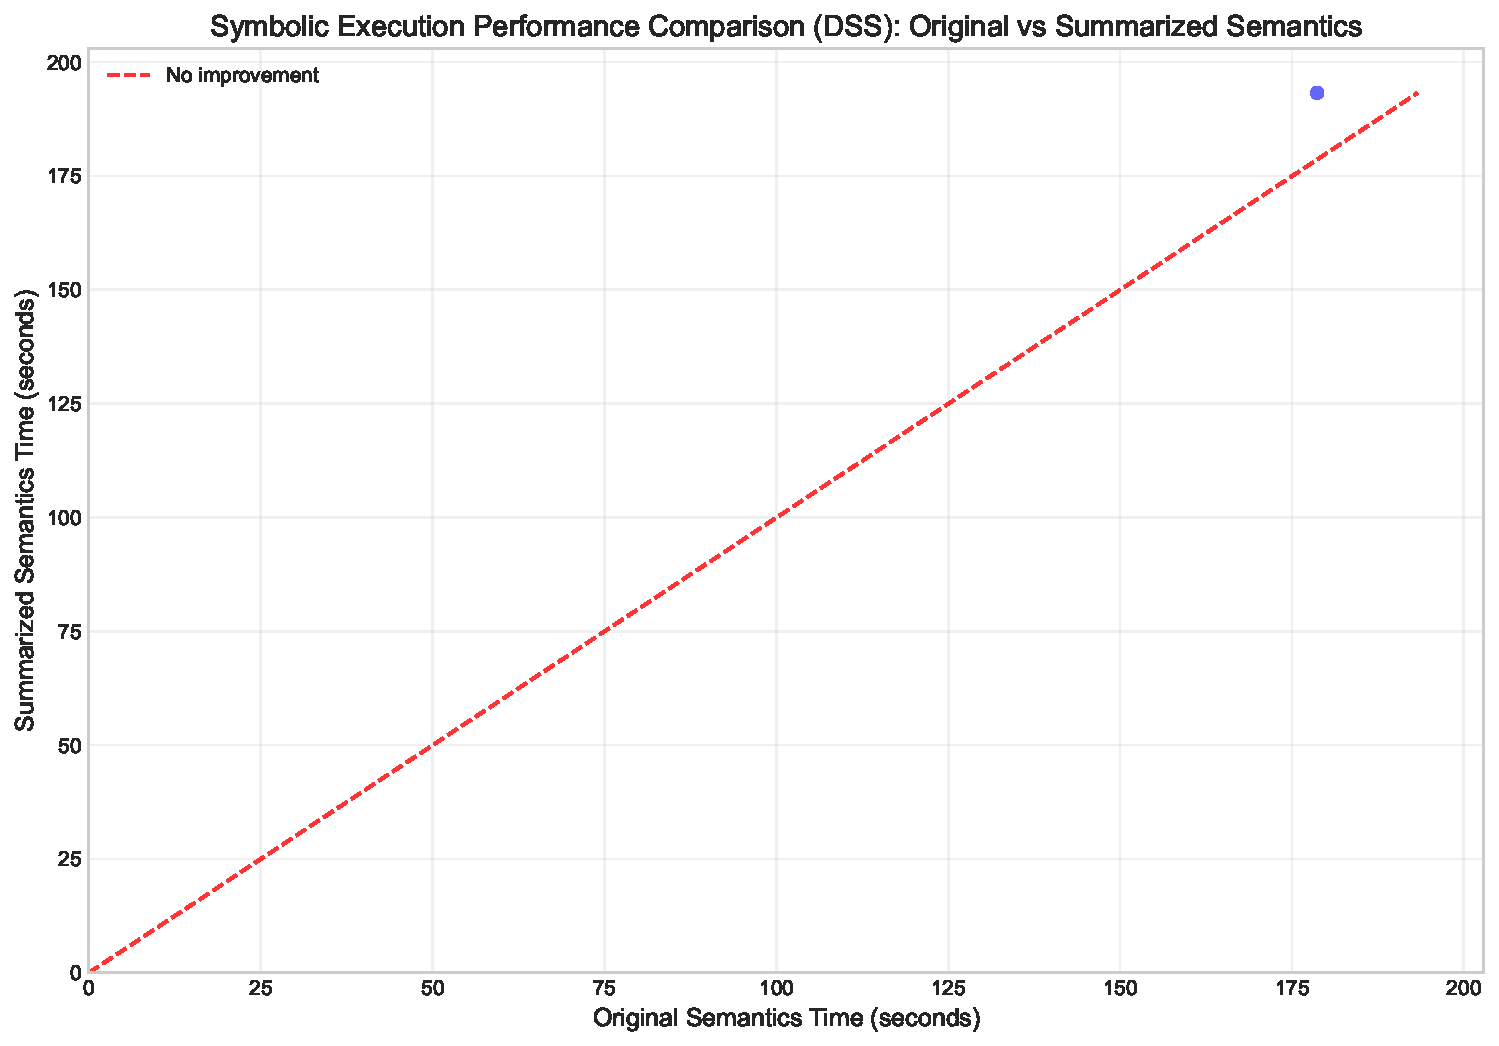
\includegraphics[width=0.8\textwidth]{charts/symbolic_dss_performance_scatter.pdf}
\caption{Symbolic Execution Performance Comparison (DSS): Original vs Summarized Semantics}
\label{fig:symbolic_dss_performance_scatter}
\end{figure}

\newpage

\subsection{Top Symbolic Test Cases by Performance Improvement (DSS)}\label{fig:symbolic_dss_test_case_improvement}

\begin{figure}[H]
\centering
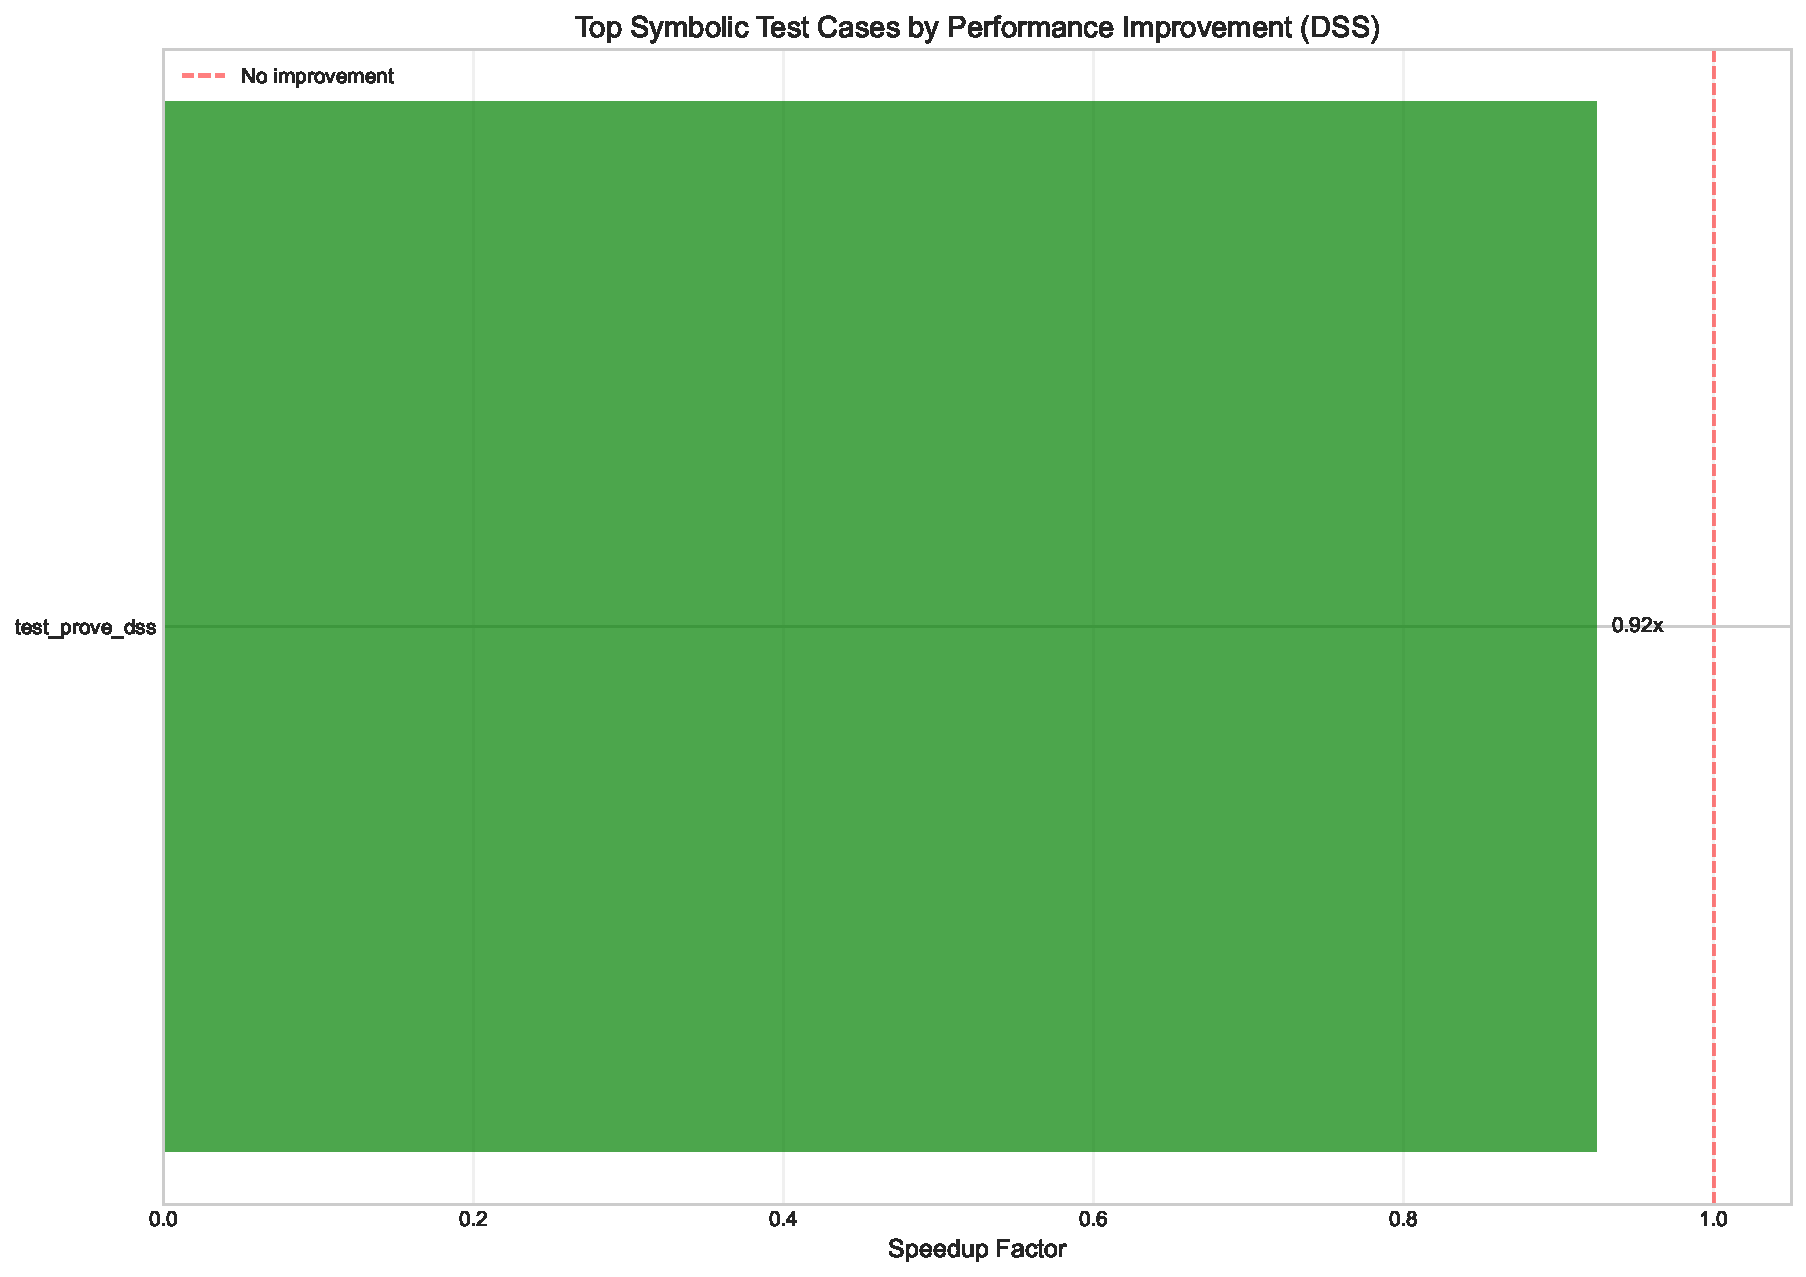
\includegraphics[width=0.8\textwidth]{charts/symbolic_dss_test_case_improvement.pdf}
\caption{Top Symbolic Test Cases by Performance Improvement (DSS)}
\label{fig:symbolic_dss_test_case_improvement}
\end{figure}

\newpage

\end{document}
